\documentclass[tikz]{standalone}

\begin{document}
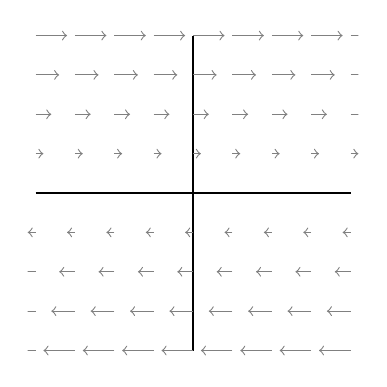
\begin{tikzpicture}[scale=0.5]
  \draw (-4, 0) -- (4, 0);
  \draw (0, -4) -- (0, 4);
  \clip (-4.2, -4.2) rectangle (4.2, 4.2);
  \foreach \x in {-4, ..., 4} {
    \foreach \y in {-4, -3, -2, -1, 1, 2, 3, 4} {
      \draw[gray, ->] (\x, \y) -- +({\y / 5}, 0);
    }
  }
\end{tikzpicture}
\end{document}
